\documentclass{article}

% if you need to pass options to natbib, use, e.g.:
% \PassOptionsToPackage{numbers, compress}{natbib}
% before loading nips_2017
%
% to avoid loading the natbib package, add option nonatbib:
% \usepackage[nonatbib]{nips_2017}

\usepackage{nips_2017}

% to compile a camera-ready version, add the [final] option, e.g.:
% \usepackage[final]{nips_2017}

\usepackage[utf8]{inputenc} % allow utf-8 input
\usepackage[T1]{fontenc}    % use 8-bit T1 fonts
\usepackage{hyperref}       % hyperlinks
\usepackage{url}            % simple URL typesetting
\usepackage{booktabs}       % professional-quality tables
\usepackage{amsfonts}       % blackboard math symbols
\usepackage{nicefrac}       % compact symbols for 1/2, etc.
\usepackage{microtype}      % microtypography
\usepackage{graphicx}

\title{Deep Learning in the Stock Market}

\author{
  Naomi Green\\
  Student at SDSMT\\
  501 East St. Joseph St. \\
  Rapid City, SD 57701 \\
  \texttt{naomi.green@mines.sdsmt.edu} \\
}

\begin{document}

\maketitle

\begin{abstract}
Predicting stock returns is something that has been attempted many times.
Everyone was looking for a better method than guess work.
When machine learning became popular the techniques were used to train a computer to recognize patterns.
Machine Learning was successful, and allowed the computer to do better at tasks the more it did them.
Neural networks, a form of machine learning have also been used, with success, but the most recent one is Deep Learning. 
Deep Learning is a neural network that has many layers of neurons, it has shown high performance in image recognition. 
This paper will focus on how deep learning has come into play in the stock market.
\end{abstract}

\section{Introduction}
The predictability of the stock market is important for investors.
They want to know that they will be making money.
There are many different algorithms that people use to try to predict how a stock will do. 
RSI(relative strength index), MACD(Moving Average Convergence/Divergence), and candlesticks are a few of the tests that can be used to tell if a stock is on an uptrend or a downtrend. 
One other way that has recently become popular is the use of machine learning models. 
This approach takes multiple factors into account when explaining the expected future stock values.

There are deep learning networks for the stock market that take into account the news.[4]
They will go and look through the current news, to see if they can get better predictions by using major events that affect the companies that have stocks.

"Experimental results show that our model can achieve nearly 6\% improvements on S\&P 500 index prediction and individual stock prediction, respectively, compared to state-of-the-art baseline methods."[4]

This was shown in the article by Xiao[4] on their model which uses this Natural Language Processing.


\subsection{Stock Market}
It may seem like the Stock Market data is so random that a neural network couldn't possibly have a chance at recognizing the patterns. 
In addition the stock market can change quickly, and a stocks value may drop off for seemingly no reason.
Since there are methods that are used to predict the stock market it would make sense that machine learning became popular with stock prediction.

\subsection{Deep Neural Networks}
There are a variety of frameworks that have been designed to work with a deep learning neural network. 
Many of the frameworks are written for python like Tensorflow, but there is also Singa in C++, and Torch in LUA among others.

Deep Learning is a part of the broad field of Machine Learning. 
It is similar to Neural Networks in that they are networks comprised of perceptrons.
In deep learning unlike neural networks though, there happens to be more than one hidden layer.
It learns multiple levels of representations, each corresponds to different levels of abstraction.
This allows the network to represent complex objects.
"Results show that deep neural networks
generally outperform shallow neural networks, and the best networks also outperform representative machine learning models."[1]


\subsection{TensorFlow}
Tensorflow is one of the frameworks designed to work with a Deep Learning Neural Network.
It runs in Python with an efficient C++ backend. 
It is open source, and usable from a variety of platforms. 
Tensorflow was the platform that is used in this papers analysis of stock data.

\subsection{Recurrent Neural Network}
Recurrent Neural Networks are designed to take advantage of sequential information.
RNNs are commonly used with language.
If you are going to try to predict a word in a sentence it helps to know what came before, and in what order.
So the RNN has a memory of a sort that keeps track of the order the values happened.
With that in mind it makes sense that the recurrent neural network would be the best suited for predicting the stock market.

What makes the RNN so different is that is is arranged in a sequence. \\


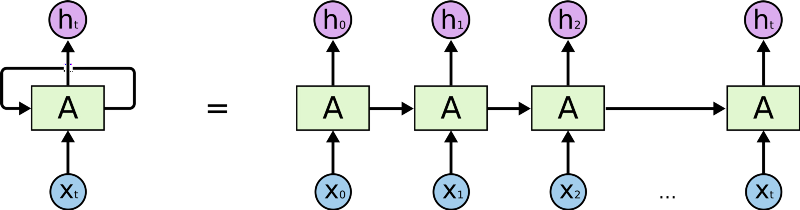
\includegraphics[width=\textwidth]{0_WdbXF_e8kZI1R5nQ.png}[8]
As shown in the diagram above each layer in a recurrent neural network is made up of the previous layers output, a bias, and the next input in the sequence.
With the diagram it is clear how the order the inputs show up matters.
With the way RNNs work the prior perceptrons have less effect on the result.
The network can only get so long before the initial input has no effect on the output.

\subsection{ReLU}
One of the more common, and simple activation function is the Rectified Linear Unit.
The ReLU function takes the value passed in, the computes the max of that value and zero.
\[f(x) = max(x, 0)\]
The only problem with the ReLU activation function is that there is a possibility that with many negative inputs everything gets zeroed out, then no training happens.

The rectified linear unit function was designed to mimic the neurons in the brain.
Neurons are either all or nothing. 
If there isn't enough input to get past the firing threshold nothing goes through.
"Research has shown that ReLUs result in much faster training for large networks."[9]
ReLUs have become popular because of that.

However the simplest solution is not always the best.
As mentioned earlier there is a chance that the whole thing ends up zeroed out.
If not used correctly you could end up with 40\% of the network dead and never activating.[9]

\section{Training}
A deep neural net consists of multiple layers of perceptrons, an input layer, multiple hidden layers, and an output layer.
For each node in the hidden layer, and output layer, the value of that node is:
\[\sum x_i * w_i\]
x is the inputs, prior layers are the inputs to the next layer. \\
w is the weight that corresponds to the input. \\
That value is then sent through the activation function for that node.

The weights connecting these layers of neurons are initialized to small random weights, and need to be trained for the optimal result.
There are a few ways to train the network, supervised training is the way that we will focus on. 

Supervised training means that for each input data set, the output is known.
The order the input data sets are run is randomized each time to make sure that the network isn't learning the order that data is sent in, but actually learning the data.
The output the network provides is then compared to the expected output, and the difference is propagated back through the network to get more accurate results.
Throughout all the iterations of testing we are trying to find the local minimum that will provide good results across the board.

\subsection{Data}
This project uses historical stock market data that dates back to 2001 to train the network. This means that the network will be trained on an uptrend, downtrend, and no trend.
This is important because if the network was only trained on when the market was having a good year it wouldn't know how to respond when the market drops.
Each stock has its own csv file that gets read in to the program.
Inside each file is the date that the information is from, the opening price, the high for the day, the low for the day, the closing price, and the volume.
The data is used as a rolling forecast.
This means that during the testing phase you have a window of say twenty days, you would start the testing using the oldest twenty days and see if it can tell you the twenty-first day.
Then you would move the window so that the twenty-first day was included and see if the program can tell you the next value.

\subsection{Testing}
Testing is also used in the training process, it consists of testing the current weights with data that wasn't used during the testing phase. 
At the end of each iteration the training loss and the testing loss can be calculated.
These values tell you how the network is working.

When tests are run the program will print out graphs every few epochs that show the expected result compared to what the program guessed. 
The graphs below are an example of what that would look like.
They are the graphs printed from epoch 11, 22, 37, and 49.
You can see that the result is changing, sometimes getting better, sometimes worse.\\	

\includegraphics[width=.5\textwidth]{AAPL_epoch11_step2097.png}
\includegraphics[width=.5\textwidth]{AAPL_epoch22_step4193.png}\\


\includegraphics[width=.5\textwidth]{AAPL_epoch37_step5233.png}
\includegraphics[width=.5\textwidth]{AAPL_epoch49_step2065.png}

The resulting weights from the training session are stored, so that the next time the program is run it doesn't need to be trained.
This is helpful, because then you can train the weights once, then each day see what it thinks the next days market will look like.


\section{The Program}
The first part of figuring out how to incorporate deep learning into predicting the stock market was researching what other people had done.
The program that was used as a starting point can be found on github[6]. 
\begin{center} \url{https://github.com/lilianweng/stock-rnn.git} \end{center}
It provides command line arguments for most of what you would want to edit in the network for better results.

I chose this one to start from because it seemed the most complete.
It was also the easiest to install and get running.
The program has options to look at a single stock, or cover all of them.
It reads the input from the csv file, then trains the network on it. 
The training data contains most of the total dataset.
The rest is in the testing data set.
The data is then sent through the tensorflow graph one batch at a time. 
Each batch is made up of the specified number of test cases. 
For each batch the the training loss is updated, the step is printed, and the samples that are to be plotted are plotted.
At the end of training the save function gets called.
This function saves the current network model in a ".model" file in the logs directory.
This file can be loaded later to run the program with those weights.

When using tensorflow each input in the graph that is being built is defined as a placeholder.
Placeholders are used to build the graph for the data.
They hold the place of where the numbers are going to be filled in later.
The hidden nodes and output node are defined by the functions that produce their result.

The program needs to be run with the same command-line options that it was trained with.
If the command-line options don't match python is unable to make sense of the file.

\subsection{Tensorboard}
Tensorboard was also running with the program. It allows interaction with the graph that tensorflow creates to run the program. It also shows the changes in variables over time. This makes it easy to see what the program is doing, and to debug possible issues. The graph currently being used is shown below.

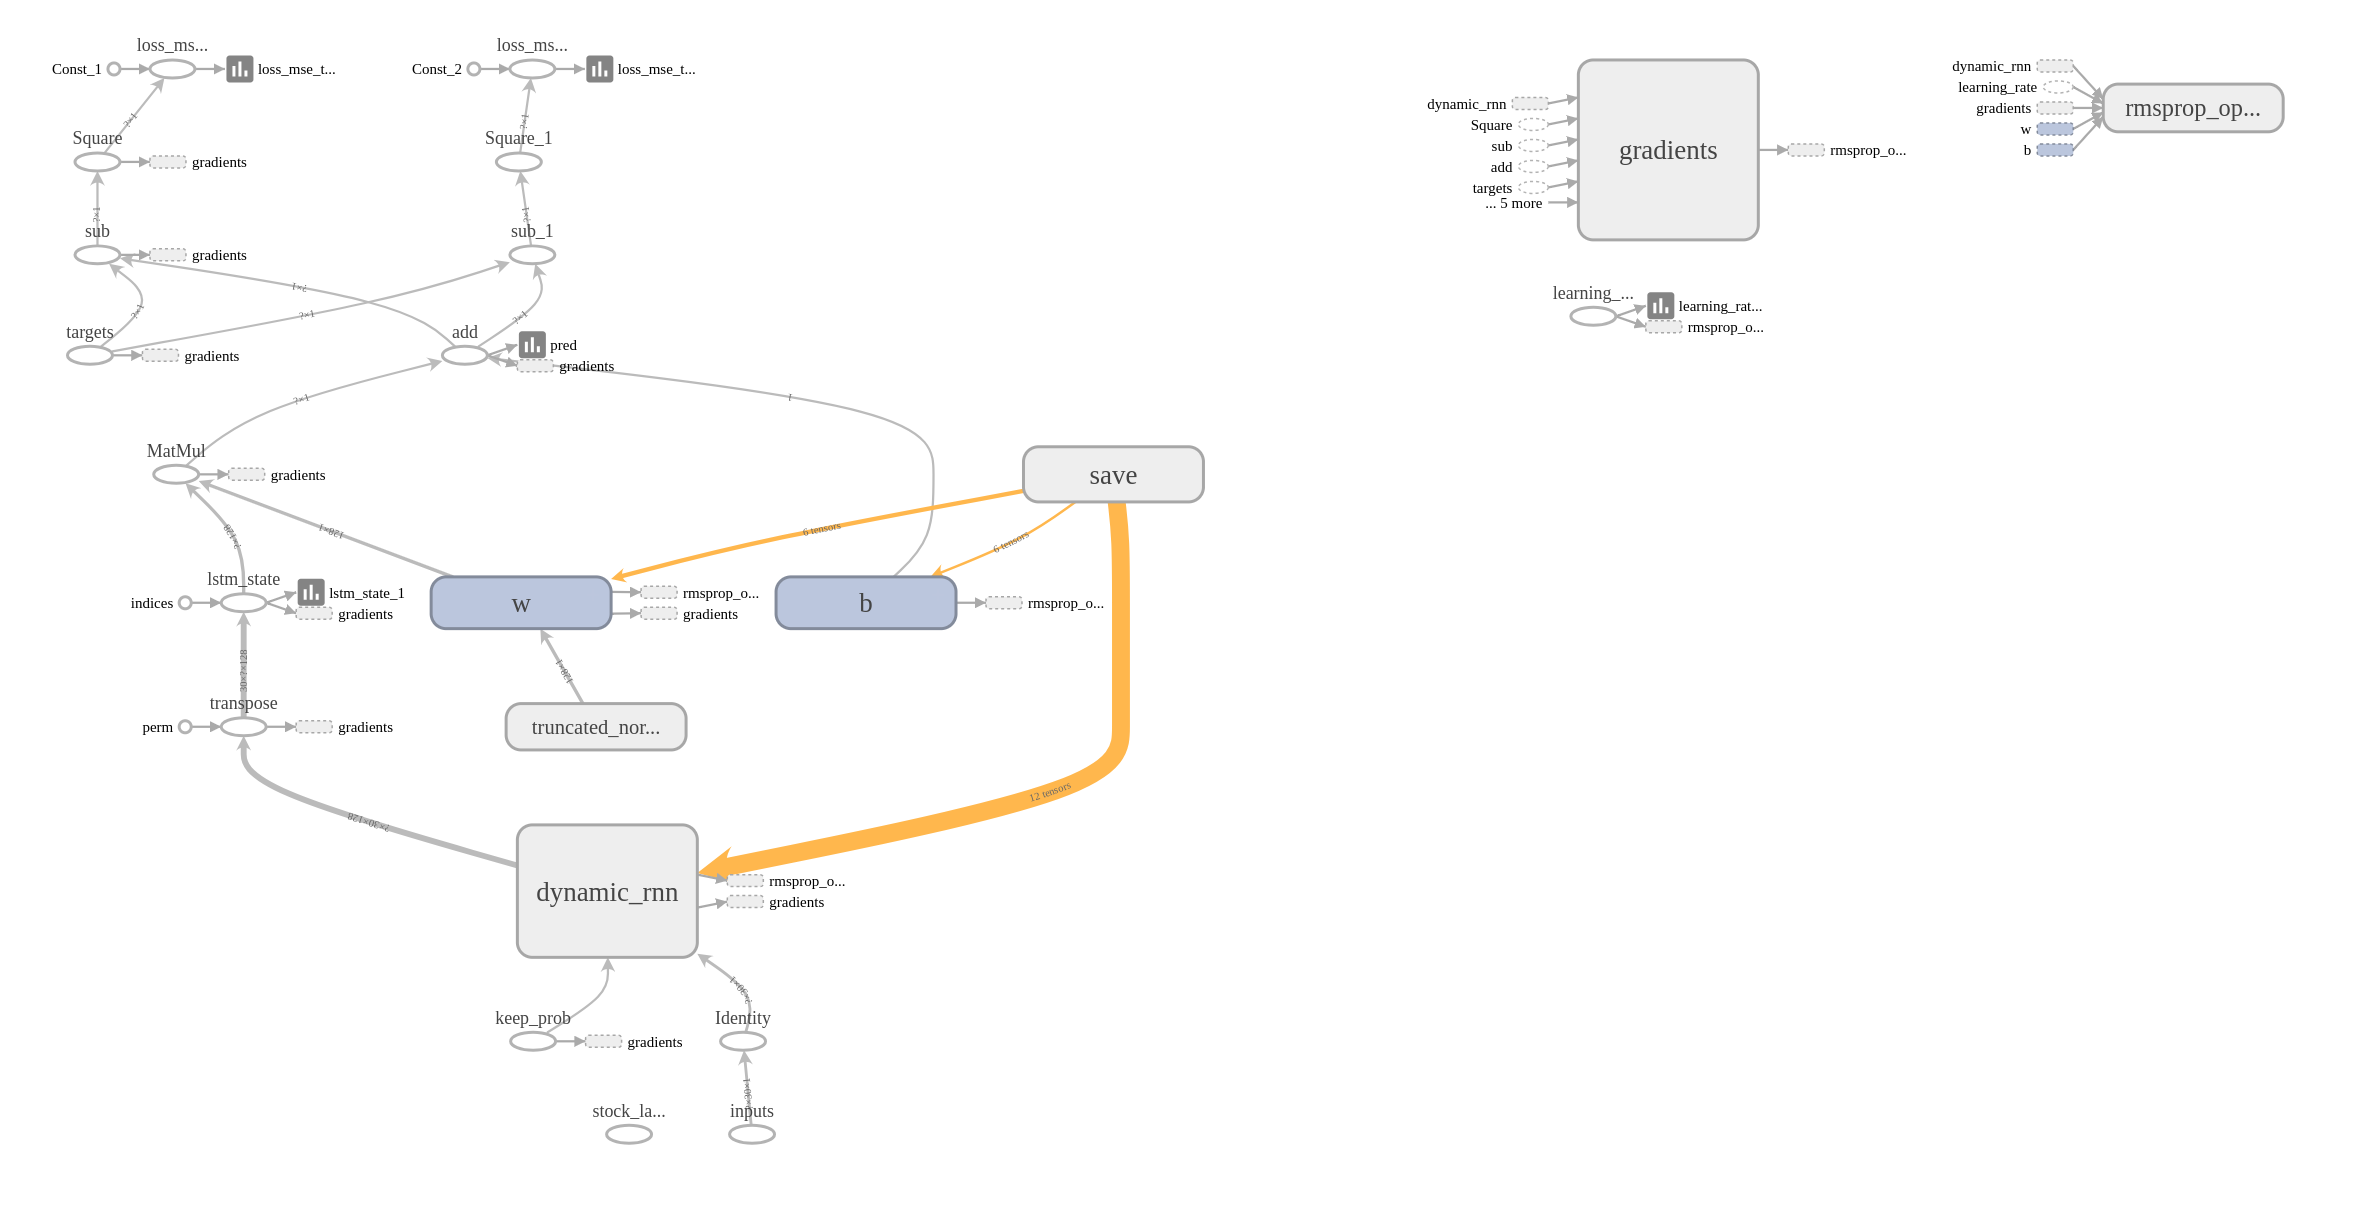
\includegraphics[width=\textwidth]{png.png}

This graph shows the whole program. Each of the rectangular boxes expands into a graph of their own. The one labeled dynamic\_RNN is the graph that calculates the result, is the neural net.

\section{Results of Running the Program}
The program was run with two hidden layers, three hidden layers, four hidden layers, and five hidden layers. 
The results are better the fewer layers there are.


The two hidden layer network performed very similar to the single layer in the graphs above. \\

\includegraphics[width=.5\textwidth]{AAPL_epoch03_step2.png}

The results from a network with three hidden layers were similar to the results with a single layer, in general there wasn't much change until it hit epoch 41(shown below). \\


\includegraphics[width=.5\textwidth]{AAPL_epoch11_step3.png}
\includegraphics[width=.5\textwidth]{AAPL_epoch41_step3.png}


The results shown below show that the network didn't learn anything useful with five hidden layers. 
This was the same with 4 hidden layers.
What it was figuring out is the median of the data.
No matter what was sent in the same number was always returned, and it looked like it was moving towards the middle of the expected data. \\


\includegraphics[width=.5\textwidth]{AAPL_epoch07_step5.png}

With a single hidden layer the training of the network took all night, with three hidden layers it took three days to run. 
When five hidden layers wasn't showing any success it was canceled. 
Based of of the tests I ran it seemed like the more layers that are used the worse it performs.

I also ran it with one hidden layer, a learning rate of .004, a batch size of 21 and learning rate decay of .9.
When the graph is printed for each epoch you can see that it gets closer to matching the line then seems to go back to where it started.
This was the settings where I got the best results yet.


\section{Conclusion}

Many of the other articles and github programs that I looked at had better results than I was getting.
Given more time I would look more into the differences between the successful programs, and the unsuccessful ones to see if I could develop one that also did reasonably well. 
With being able to modify everything, it makes it hard to find the right combination.


Tensorflow is very flexible, and allows a lot of control in how the network is layed out and runs.
There are a lot of variables in the deep learning network that weren't touched at all. 
This deep learning model still has a lot of room for improvement in learning to predict how stocks will do.

Other variables that could change to affect the accuracy are the initialization and activation scheme, and early stopping.
Changing the design of the perceptrons and layers produced drastically different results. 
Different kinds of neural networks might get better results as well.
While this program used a Recurrent Neural Network, a Convolutional neural network, or another might be better suited to predicting stocks. 

It isn't possible to find the "best" setup for the job, and there is no universal deep neural network.
The best that can be hoped for is finding a setup that gets the job done well.

While I learned a lot through modifying the code, and testing it, I have found that there is a lot more to learn that I haven't even touched yet. 



\section*{References}
\medskip

\small

[1] Abe, Masaya and Hideki Nakayama. “Deep Learning for Forecasting Stock Returns in the Cross-Section.” CoRR abs/1801.01777 (2017): n. pag.

[2] Heinz, Sebastian. “A Simple Deep Learning Model for Stock Price Prediction Using TensorFlow.” Medium, ML Review, 9 Nov. 2017, medium.com/mlreview/a-simple-deep-learning-model-for-stock-price-prediction-using-tensorflow-30505541d877.

[3] Perry, Tal. “Deep Learning the Stock Market – Tal Perry – Medium.” Medium, Medium, 3 Dec. 2016, medium.com/@TalPerry/deep-learning-the-stock-market-df853d139e02.

[4] Ding, Xiao\ \& Yue Zhang\ \& Ting Liu\ \& Junwen Duan “Deep Learning for Event-Driven Stock Prediction” (2015)

[5] Liew, Jim Kyung-Soo and Mayster, Boris, Forecasting ETFs with Machine Learning Algorithms (January 14, 2017). Available at SSRN: https://ssrn.com/abstract=2899520 or http://dx.doi.org/10.2139/ssrn.2899520

[6] https://github.com/lilianweng/stock-rnn.git

[7] Britz, Denny. “Recurrent Neural Networks Tutorial, Part 1 – Introduction to RNNs.” WildML, 8 July 2016, www.wildml.com/2015/09/recurrent-neural-networks-tutorial-part-1-introduction-to-rnns/.

[8] Ma, Jianqiang. “All of Recurrent Neural Networks – Jianqiang Ma – Medium.” Medium, Medium, 2 Apr. 2016, medium.com/@jianqiangma/all-about-recurrent-neural-networks-9e5ae2936f6e.

[9] Kulbear. “Kulbear/Deep-Learning-Nano-Foundation.” GitHub, github.com/Kulbear/deep-learning-nano-foundation/wiki/ReLU-and-Softmax-Activation-Functions.

\end{document}
